\chapter{\textit{On-line} HDF}\label{ch:prepost}

Sin dalla prima introduzione della terapia dialitica, si è cercato di sfruttare sia la diffusione che la convezione come fenomeni fisici per la purificazione del sangue. È del 1967 il primo articolo sull'uso dell'ultrafiltrazione e della diluizione del sangue come metodi dialitici. Nel 1969 si teorizzò la possibile applicazione simultanea di diffusione e convezione in dialisi e otto anni più tardi, nel 1977, H. Leber mise in pratica quelle teorie, pubblicando il primo articolo in cui si coniava il termine \textit{emodiafiltrazione} \cite{bib:history}.

L'emodiafiltrazione (acronimo HDF) è un trattamento dialitico più efficace dell'emofiltrazione e dell'emodialisi, grazie soprattutto alla simultaneità di diffusione e convezione, che rende possibile la rimozione di soluti sia a basso peso molecolare (diffusione) che a medio-alto peso molecolare (convezione). Inoltre, i sintomi tipicamente indotti dalla dialisi (pirogenicità, ipotensione, crampi) risultano essere meno frequenti in HDF \cite{canaud}. Esistono quindi almeno due vantaggi con l'utilizzo dell'HDF:
\begin{itemize}
\item ampliamento del range dei pesi molecolari delle tossine uremiche rimosse;
\item miglioramento della biocompatibilità del trattamento dialitico, con riduzione degli effetti negativi a lungo termine della dialisi.
\end{itemize}
Nei prossimi paragrafi 
verrà spiegato il significato del termine \textit{on-line} quando ci riferisce all'HDF e si descriveranno le modalità di \textit{pre-diluizione}, \textit{post-diluizione} e \textit{diluizione mista}, confrontandone i pro e i contro relativamente all'efficacia nella rimozione delle tossine uremiche.

\section{\textit{On-line} HDF}
L'\textit{on-line} HDF è stata introdotta principalmente per contenere i costi del liquido di reinfusione rispetto all'HDF classica, in cui tale liquido era fornito in sacche sterili e in quantità limitate. Col termine \textit{on-line} ci si riferisce pertanto alla produzione sul luogo e al momento del liquido da reinfondere nel paziente.

L'HDF condivide con le altre modalità dialitiche il sistema di ultra-purificazione dell'acqua e il circuito idraulico che miscela l'acqua ultra-pura con opportune soluzioni concentrate al fine di ottenere il fluido da convogliare al dializzatore. La particolarità dell'HDF (e dell'HF) è quella di possedere, a valle del sistema di miscelamento, un filtro in più (filtro per la \textit{cold sterilization}) che garantisce la non pirogenicità e in generale l'emo-compatibilità del fluido che sarà iniettato direttamente nel compartimento ematico per la diluizione (\figurename~\ref{fluido}, \figurename~\ref{circuito}). Con la semplice aggiunta di questo filtro l'HDF perde quel vincolo, cioè quello dell'uso ``parsimonioso'' della diluizione, che impediva di sfruttare al massimo delle loro potenzialità i fenomeni di trasporto convettivi.
\begin{figure}[htb]
	\centering
		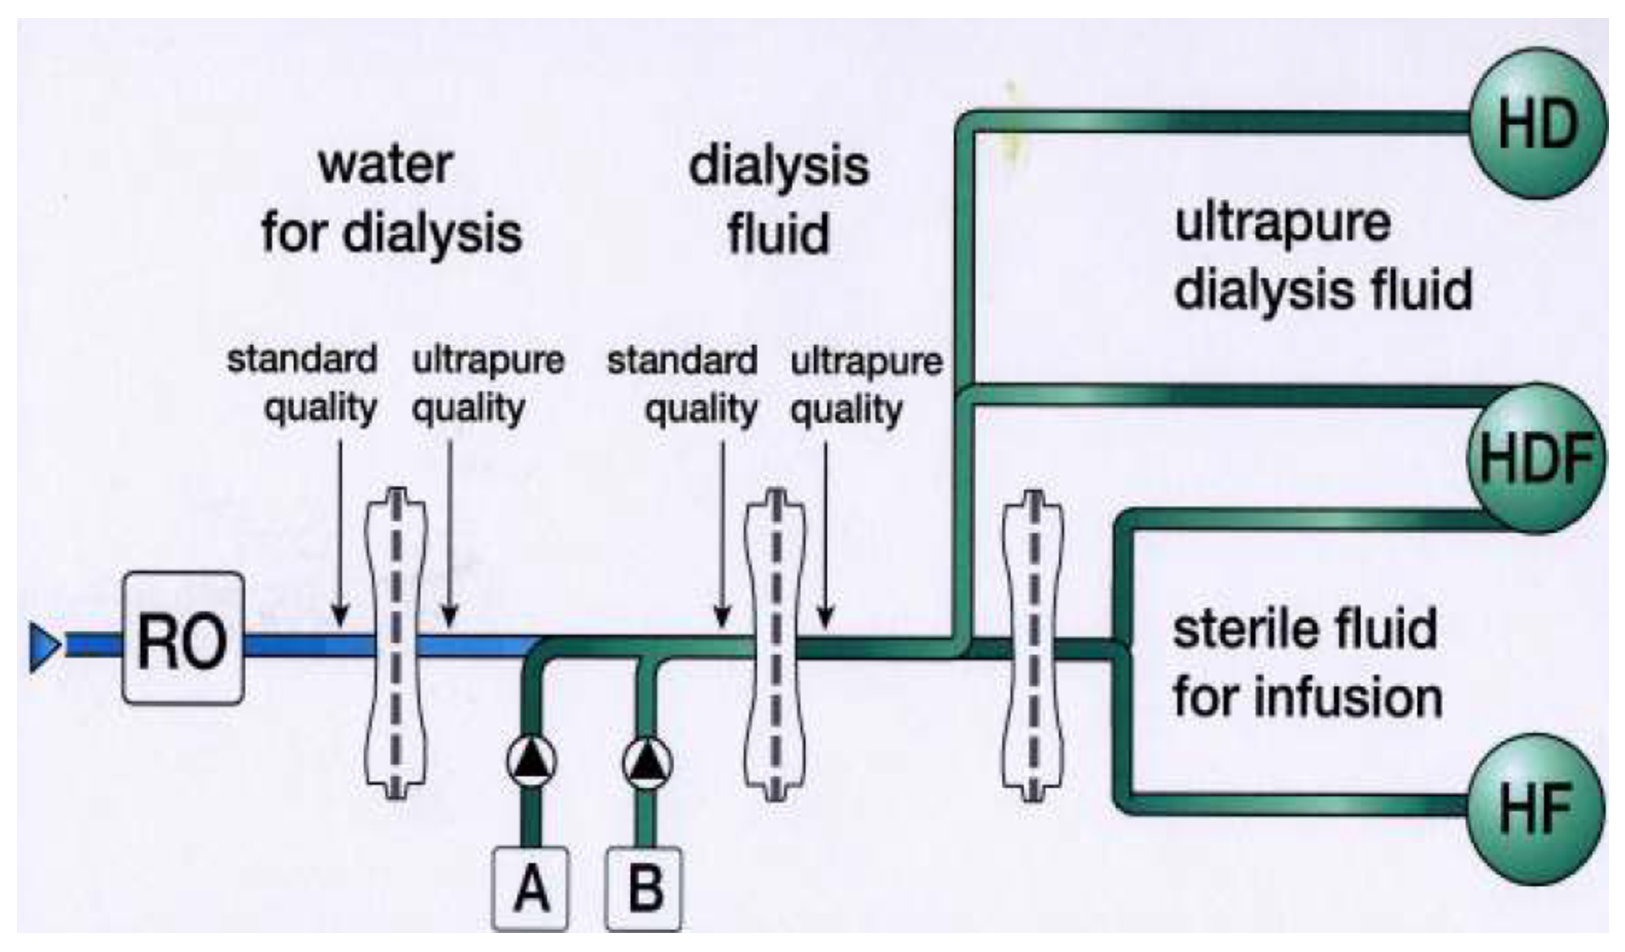
\includegraphics[width=0.6\textwidth]{immagini/NIC/fluido.eps}
		\caption{circuito di produzione del dialisato e del liquido di sostituzione durante varie tipologie di dialisi.}\label{fluido}
\end{figure}

L'acqua, che deve essere processata ed utilizzata nel circuito di dialisi, passa attraverso una fase di pretrattamento e una fase di dissalazione per osmosi inversa (RO), al fine di creare acqua ultra-pura che rientri nelle seguenti caratteristiche: per ogni millilitro batteri per un massimo di $100$ unità formanti colonie ed endotossine inferiori a $0.25$ unità (\figurename~\ref{acqua}). 
\begin{figure}[htb]
	\centering
		\fbox{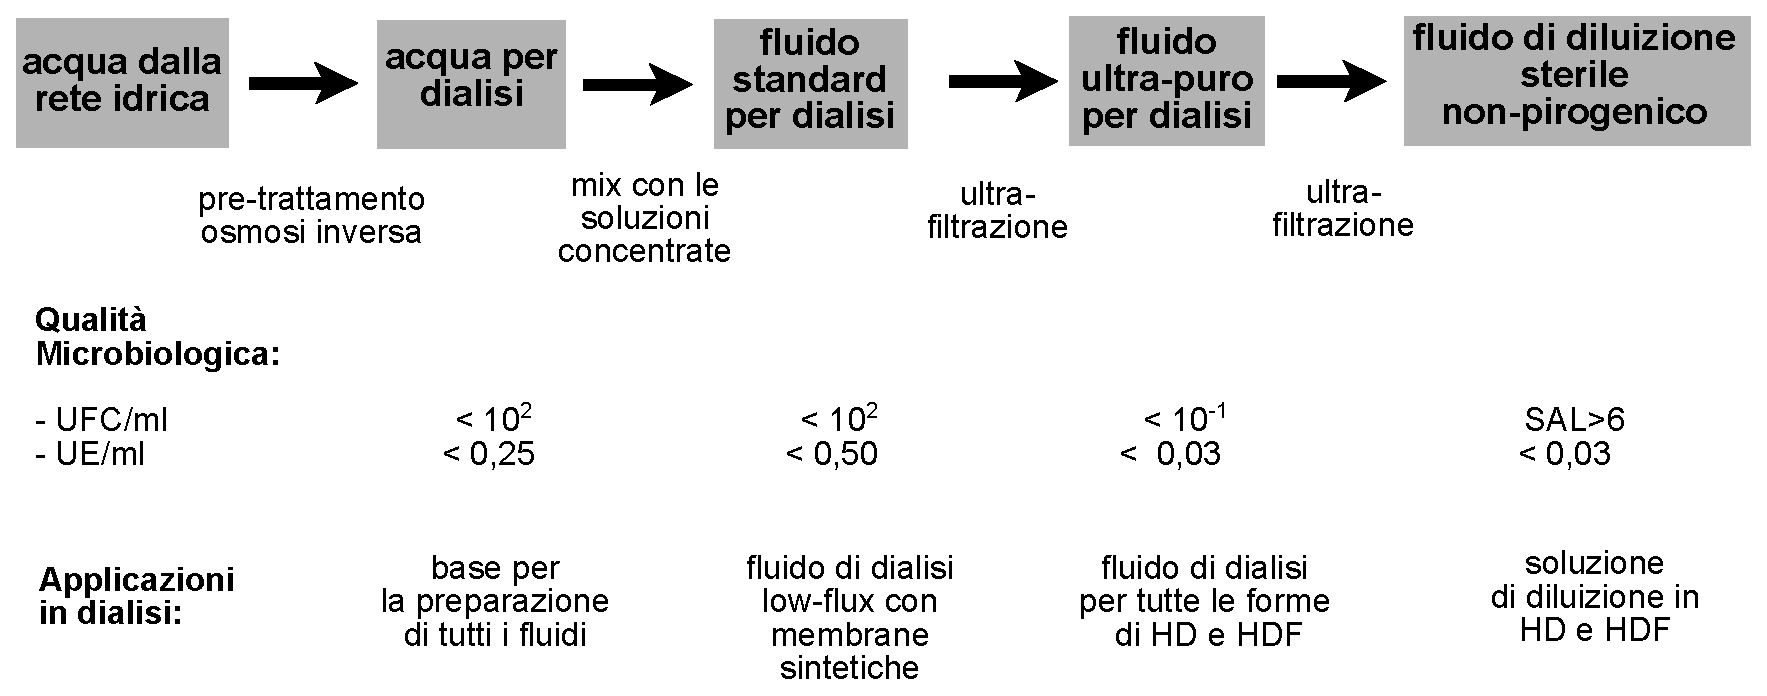
\includegraphics[width=0.9\textwidth]{immagini/NIC/acqua.eps}}
		\caption{processo di preparazione del liquido di dialisi, partendo da semplice acqua fino alla creazione di liquido sterile e non pirogenico. Il termine CFU sta per \textit{colony-forming units}, EU per \textit{endotoxin units} e SAL per \textit{sterility assurance level}}\label{acqua}
\end{figure}
Il trattamento tramite osmosi inversa oltre a fornire acqua ultra pura è anche un'eccellente barriera verso i principali contaminanti chimici e batterici. Il passo successivo è quello della preparazione del liquido di dialisi che si ottiene miscelando l'acqua ultrapura con i concentrati acidi e basici. Dopo la miscelazione c'è un ulteriore ultrafiltrazione prima che il liquido di dialisi possa essere convogliato verso il filtro dializzatore.
Nel caso di HDF o HF vi è ancora un altro filtro che dà al liquido di dialisi le caratteristiche per poter essere infuso nel compartimento ematico. La reinfusione, o diluizione, è gestita via software per mezzo di una pompa roller e di una valvola per la selezione di pre- o post-diluizione. L'utilizzo di due filtri, e addirittura tre per la tecnologia sviluppata da Gambro, è quindi necessario per ottenere una purificazione ottimale del liquido di dialisi affinché possa essere immesso, senza rischi, direttamente nel compartimento ematico del paziente \cite{bib:tech}.
\begin{figure}[htb]
	\centering
		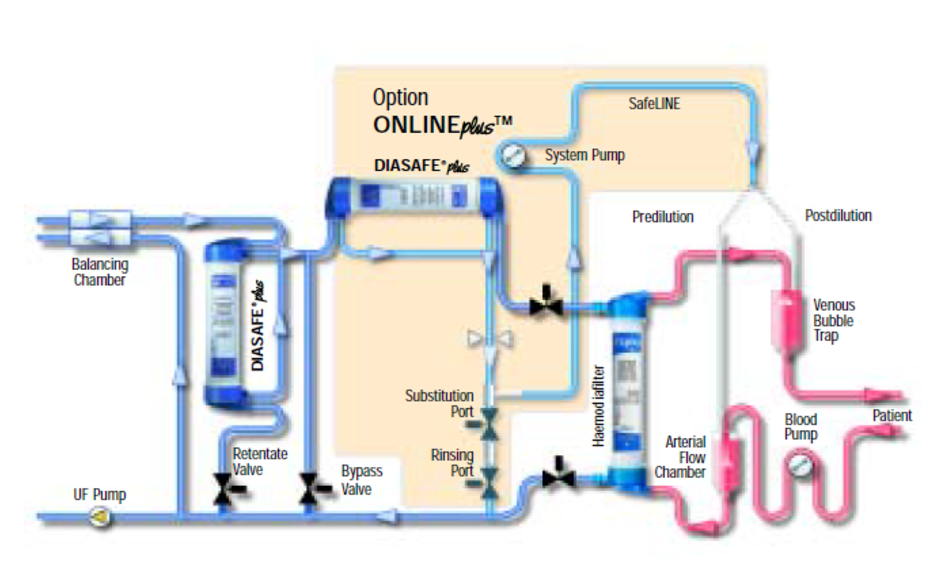
\includegraphics[width=0.7\textwidth]{immagini/NIC/circuito.eps}
		\caption{circuito di produzione di dialisato e liquido di sostituzione durante una seduta di on-line HDF}\label{circuito}
\end{figure}

Con l'introduzione dell'HDF sono sorti numerosi interrogativi, in particolare riguardo al metodo di diluizione da preferire (pre \textit{vs} post) \cite{masakane, colussi}. Nei prossimi paragrafi si indicheranno i vantaggi e gli svantaggi delle differenti modalità di diluizione disponibili per l'HDF.

\section{Emodiafiltrazione con pre-diluizione}
In questa modalità di HDF il liquido di diluizione è miscelato al sangue prima che questo entri nel filtro dializzatore (\figurename\ref{pre}), migliorandone le proprietà reologiche e abbassando a tal punto la probabilità di coagulazione del sangue, da richiedere dosi di eparina minori (o addirittura nulle) rispetto ad altri tipi di dialisi. 
\begin{figure}[htb]
	\centering
		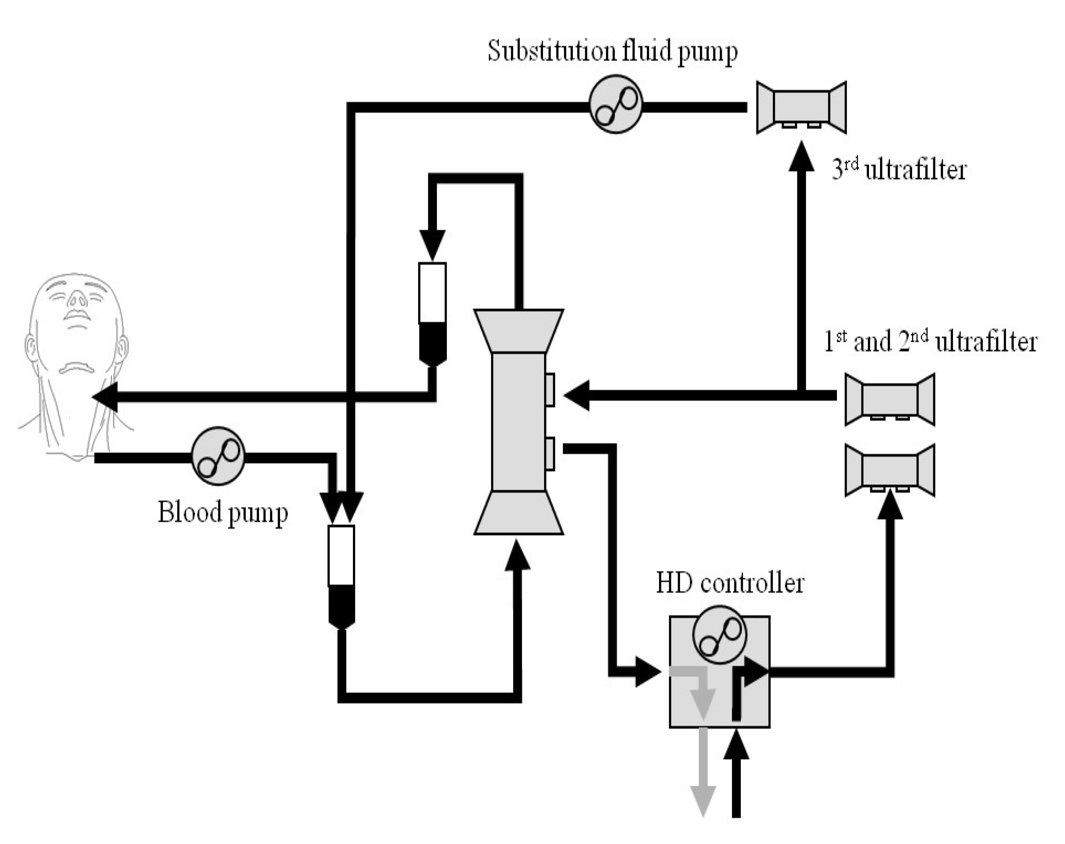
\includegraphics[width=0.7\textwidth]{immagini/NIC/pre.eps}
		\caption{circuito dell'on-line HDF tramite pre-diluizione. Il fluido di sostituzione sterile viene prodotto on line dal dialisato tramite tre filtri; questo viene in seguito reinfuso pre-filtro tramite l'utlizzo di una pompa.}\label{pre}
\end{figure}
Permette inoltre di effettuare ultrafiltrazioni spinte anche in pazienti con portate ematiche (da fistola o da catetere centrale) basse o con alto ematocrito, senza che pressioni di trans-membrana\footnote{per pressione di trans-membrana si intende la differenza di pressione a cavallo della membrana del dializzatore necessaria all'estrazione dei fluidi dal compartimento ematico.} (TMP) troppo alte riducano l'efficenza del dializzatore. Con la pre-diluizione si verifica una diminuzione dell'efficacia del fenomeno diffusivo. Questo accade perchè i soluti uremici nel dializzatore, essendo diluiti, presentano tra lato sangue e lato dialisato un gradiente di concentrazione (la forza motrice della diffusione) ridotto. Gli alti volumi di reifusione, nonostante la ridondanza dei sistemi filtranti, aumentano a lungo termine il rischio di contaminazione da sostanze nocive, potenzialmente presenti nei fluidi utilizzati per la miscela dialitica. Inoltre ad alti volumi di reinfusione seguono necessariamente alte portate di ultrafiltrazione\footnote{se così non fosse nell'organismo si avrebbe un accumulo di fluidi fino a $40$ litri, incompatibile con la vita.} che potrebbero trascinare, oltre alle tossine uremiche, anche sostanze utili all'organismo come vitamine e oligoelementi \cite{colussi}.

\section{Emodiafiltrazione con post-diluizione}
In questa modalità di HDF il liquido di diluizione è miscelato al sangue dopo che questo è uscito dal filtro dializzatore e prima che venga reimmesso nel paziente. Essendo il sangue in ingresso al dializzatore non pre-diluito, il fenomeno diffusivo non subisce deterioramenti. Tuttavia, rispetto alla pre-diluizione, c'è il rischio che a causa dell'ultrafiltrazione comunque alta, l'emoconcentrazione lungo i capillari del filtro arrivi a tal punto da generare emolisi e coaguli. I coaguli, otturando i capillari del dializzatore, rendono necessario, a parità di ultrafiltrazione impostata, l'uso di una TMP più elevata, con conseguente aumento di probabilità di otturazione dei capillari superstiti. L'aumento della TMP può anche portare ad una perdita di proteine per adsorbimento sulla membrana del dializzatore (lato sangue), fenomeno che oltre a costituire un problema per il paziente (in quanto ne altera il bilancio osmotico) fa aumentare ulteriormente la TMP rischiesta per la dialisi, creando così un circolo vizioso che termina con l'otturazione completa del filtro.

In uno studio effettuato da Meert et al. \cite{bib:meert} si è fatta una comparazione fra diverse strategie convettive, analizzando l'efficacia della rimozione di soluti diversi. La valutazione è stata fatta basandosi su tre quantità: l'evoluzione temporale della concentrazione dei soluti in ingresso e uscita dal dializzatore (\figurename\ref{prevspost}), il rapporto di riduzione ($RR=(C_{start}-C_{end})/C_{end}$) dopo quattro ore dall'inizio del trattamento e la clearance istantanea dopo un'ora. La pre- e la post-diluizione sono state paragonate utilizzando la stessa portata di sangue, la stessa durata della seduta e stesso volume di liquido reinfuso e ultrafiltrato.
\begin{figure}[!htb]
	\centering
		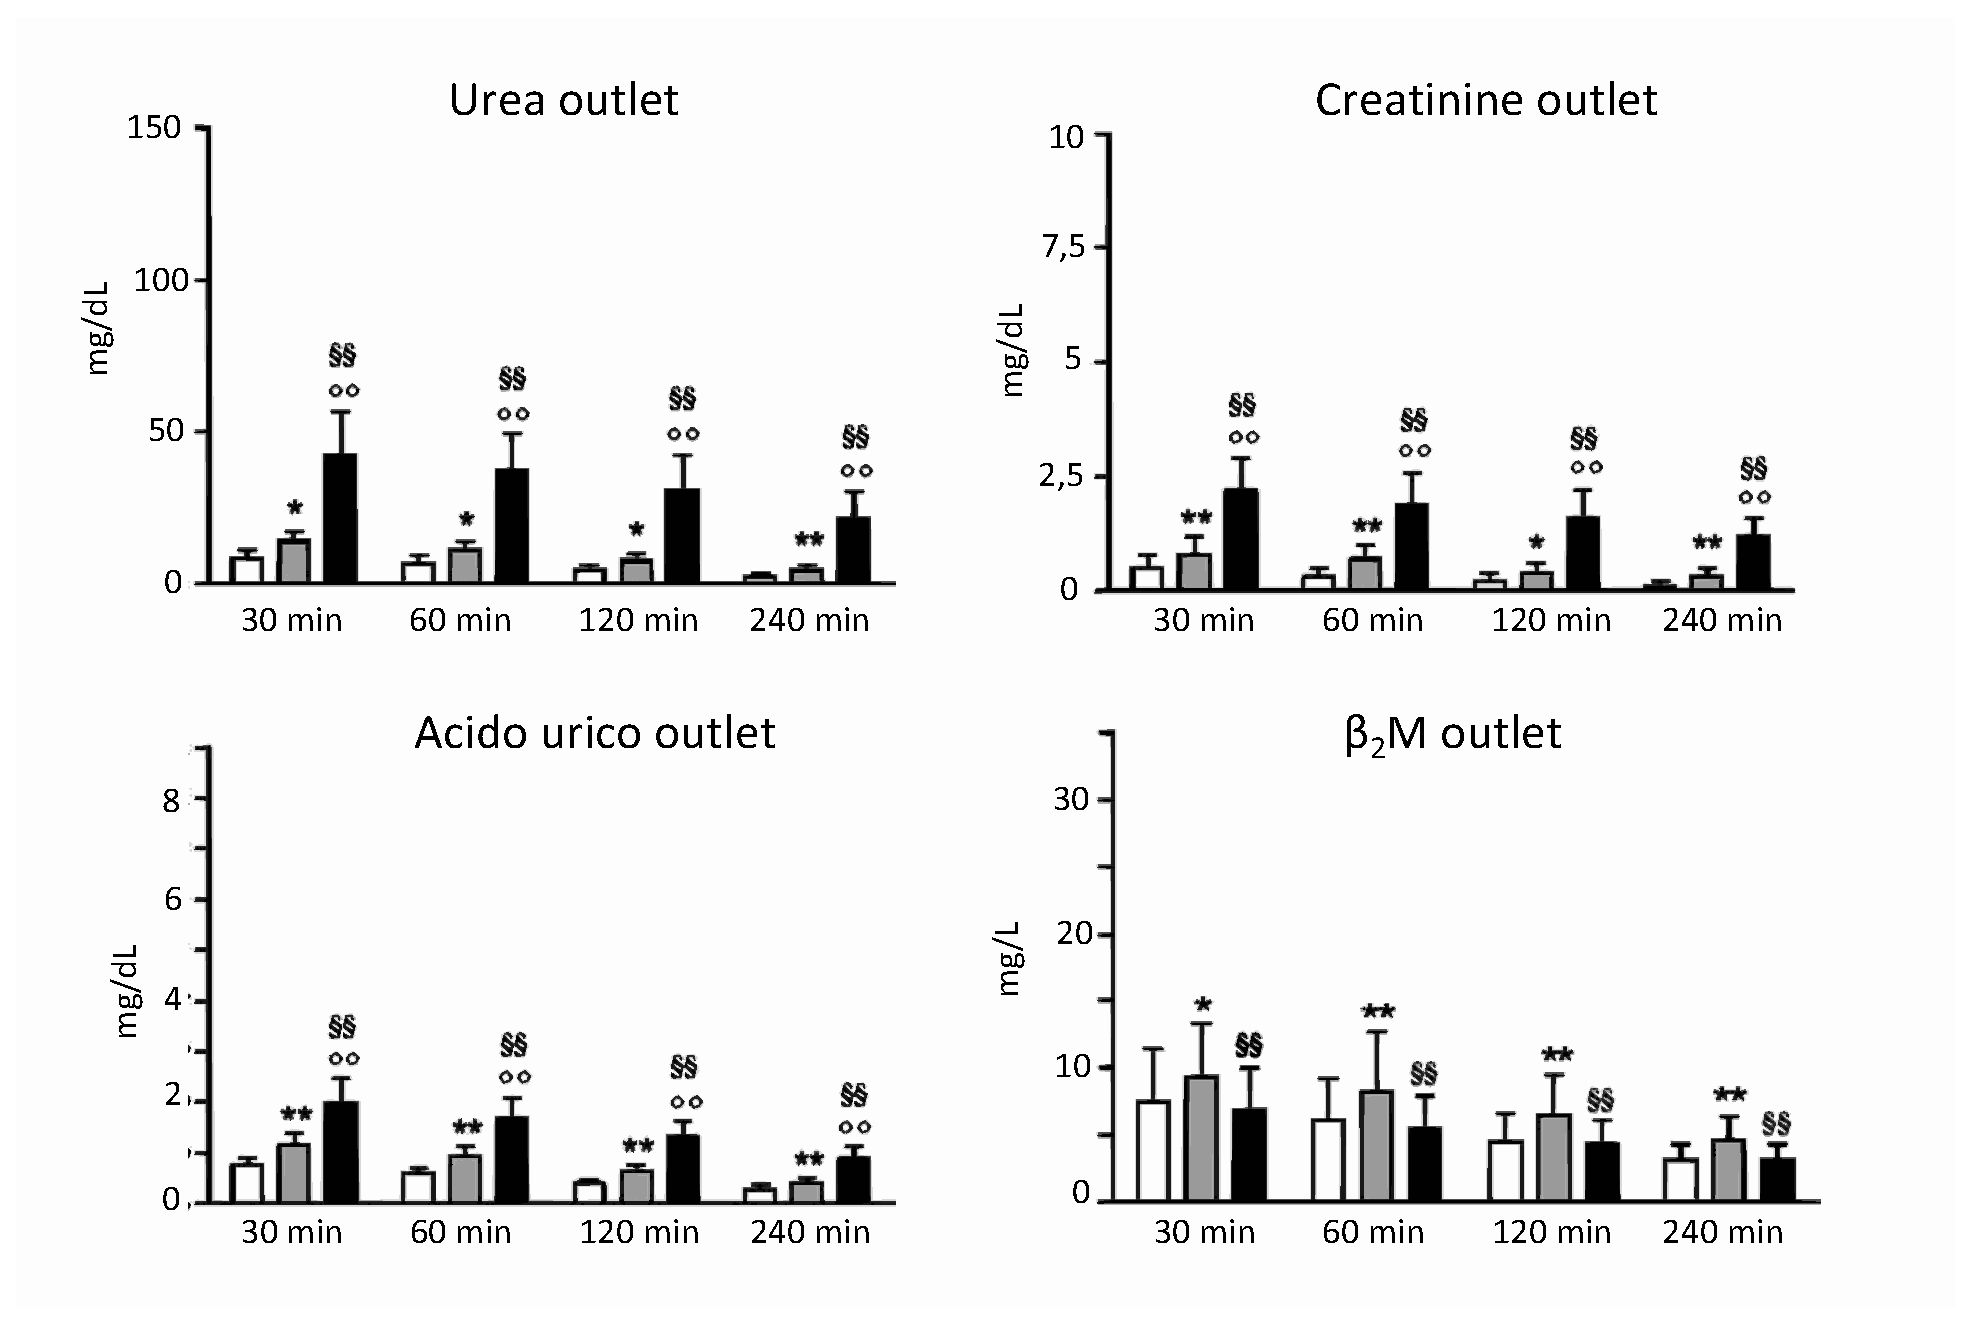
\includegraphics[width=0.9\textwidth]{immagini/prevspost_NIC.eps}
		\caption{Evoluzione delle concentrazioni in uscita dal dializzatore di alcuni soluti a differenti istanti di tempo. Barre bianche: Post-HDF; barre grigie: pre-HDF; barre nere: pre-HF. Nel caso della post-HDF il capionamento è stato eseguito a valle della diluizione. Simbolo singolo $P<0,0172$; simbolo doppio $P<0,001$. (*) pre-HDF \textit{vs} post-HDF; ($\circ$) pre-HF \textit{vs} post-HDF; (\textsection) pre-HF \textit{vs} pre-HDF.}\label{prevspost}
\end{figure}
Nei grafici in \figurename\ref{prevspost} sono mostrati i valori di concentrazione di alcuni soluti all'uscita dal dializzatore. Se ci concentriamo sulle barre di color bianco, rappresentanti la post-diluizione, e quelle grigie, riferite alla pre-diluizione, si osserva come la capacità di estrazione sia sempre più elevata con la post-diluizione. Possiamo estendere questo risultato affermando che lo stesso accade anche per altre molecole a basso e a medio peso molecolare. Quindi sembra che la post-diluizione abbia, rispetto alla pre-diluizione, una capacità estrattiva maggiore.

\section{Emodiafiltrazione a diluizione mista}
Sebbene esistano sul mercato macchine dializzatrici in grado di eseguire cicli a diluizione mista (\textit{mixed}-HDF), il loro uso non è ancora popolare; tuttavia in ambito sperimentale sono già state eseguite delle procedure dialitiche di \textit{mixed}-HDF \cite{pedrini, pedrini2, pedrini3}.
Questa nuova metodica nasce principalmente con lo scopo di raggruppare i vantaggi che la pre- e la post-diluizione possiedono singolarmente, contenendo però i rispettivi svantaggi.

Tra i criteri per stabilire in che modo la portata di diluizione totale debba essere divisa fra pre- e post-diluizione vi è quello di mantenere la frazione di filtrazione ($FF$, cioè il rapporto fra liquido filtrata dal dializzatore e liquido in ingresso) al più alto valore possibile (solitamente intorno a $0,5$), di stabilire un range in cui contenere la TMP (solitamente tra $250$ e $300$ $mmHg$) e di implementare un sistema a feedback che dirotti una piccola quantità di fluido verso la pre-diluizione, nel caso la TMP superi il valore massimo, e verso la post-diluizione se scende a valori inferiori al limite impostato. Nel primo caso, l'aumento di pre-diluizione farà diminuire la $FF$ e la TMP, riportandola nel range di ammissibilità; nel secondo caso, l'aumento di post-diluizione sarà fatto a spese della pre-diluizione, facendo aumentare così la $FF$ e la TMP, riportandola nuovamente nel range di ammissibilità. Il meccanismo appena descritto è rappresentato in \figurename\ref{tmp}.
\begin{figure}[htb]
	\centering
		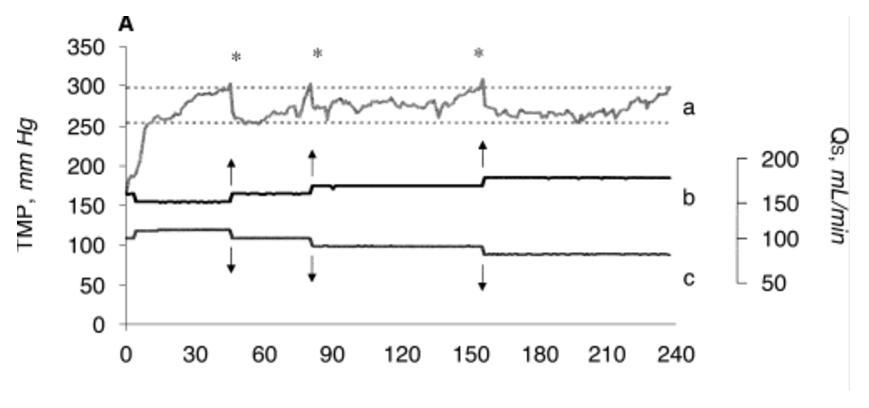
\includegraphics[width=0.8\textwidth]{immagini/NIC/tmp.eps}
		\caption{Linea a: rappresentazione grafica dell'andamento della pressione transmembrana in una seduta di HDF. La linea b descrive l'andamento della portata infusa in pre diluizione, la c invece quella in post. Ogni qualvolta la TMP supera i valori soglia viene aumentata la portata di infusione in pre diluizione così da stabilizzare la pressione attorno a valori sicuri.}\label{tmp}
\end{figure}
Riassumendo, questo sistema di controllo a diluizione mista nasce con l'intento di ottenere, durante la seduta, la più alta FF possibile, compatibilmente con la reologia locale, in modo da massimizzare la rimozione dei soluti.
Gli studi effettuati su questa tipologia di HDF  ne hanno mostrato le potenzialità e la fattibilità \cite{pedrini, pedrini2, pedrini3}.
Nel lavoro presentato da Pedrini e De Cristofaro \cite{pedrini3}, si è studiato l'effetto della \textit{mixed} HDF nel rimuovere soluti di medie dimensioni.
\begin{figure}[htb]
	\centering
		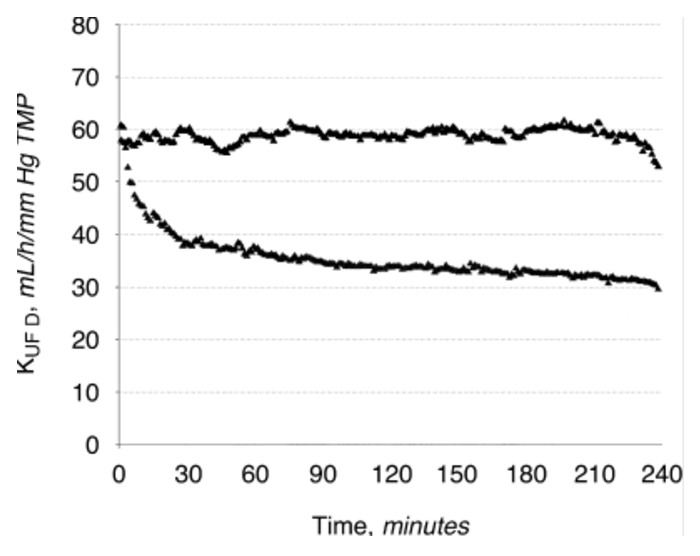
\includegraphics[width=0.5\textwidth]{immagini/NIC/idraulico.eps}
		\caption{Comportamento del coefficiente di ultrafiltrazione del dializzatore $K_{uf,D}$. Questo valore è calcolato dal rapporto della $Q_{UF}$ e la pressione transmembrana media. Viene utilizzato per valutare le modifiche istantanee della permeabilità della membrana durante la seduta. La curva superiore rappresenta la seduta di mixed HDF mentre quella inferiore la seduta di post HDF.}\label{idraulico}
\end{figure}
Oltre a limitare il deterioramento delle caratteristiche idrauliche della membrana dializzatrice (\figurename\ref{idraulico}), si è mostrato che questa tecnologia sembra migliorare le capacità depurative dell'HDF sfruttando al massimo il meccanismo di rimozione dei soluti per convezione. Inoltre, l'alta biocompatibilità dovuta all'uso di membrane sintetiche e di dialisato e fluido di sostituzione ultra puro, tipiche dell'HDF in generale, combinato con la capacità particolarmente efficace della \textit{mixed} HDF di rimuovere molecole sia a basso che a medio/alto peso molecolare, sembrano inidicare la \textit{mixed} HDF come un'efficace strategia in grado di evitare le complicazioni a lungo termine che caratterizzano le tradizionali metodologie dialitiche. Queste ricerche sono ancora agli albori e non c'è ancora stato alcuno studio multicentrico con un ampio campione statistico di pazienti per poter fare delle affermazioni certe su quale tecnica sia effettivamente la migliore. Bisognerà  anche stabilire se l'uso di frazioni di filtrazione troppo spinte possano rimuovere, oltre alle tossine, anche soluti utili all'organismo e in questo caso reinfondere i soluti utili con metodiche di tipo autologo \cite{bib:wratten} oppure reinfondendoli con preparati chimici opportuni.

\section{Stato dell'arte sulla modellistica HDF}\label{sec:stato}
In Ursino et al. \cite{ursino3} è descritto un modello matematico per l'emodiafiltrazione con rigenerazione on-line dell'ultrafiltrato (HFR). Si tratta di una tecnica analoga alla \textit{paired filtration}\footnote{nella \textit{paired filtration} (\textsection~\ref{sub:dialisi}) ci sono due filtri posti in serie: il primo è un emodiafiltro, cioè un filtro per HDF, e il secondo è un filtro per emodialisi. La diluizione avviene fra i due filtri.} ma, a differenza di questa, nell'HFR tutto l'ultrafiltrato in uscita dall'emodiafiltro è usato per diluire il sangue in ingresso all'emofiltro, così che non ci sia bisogno di ulteriori fluidi per la diluizione forniti dall'esterno. La vera ultrafiltrazione avviene nell'emofiltro, secondo le dinamiche dell'emodialisi. Il vantaggio di questa tecnica consiste nell'utilizzare un fluido di diluizione autologo, che viene rigenerato prima della sua reimmissione nel circuito attraverso il passaggio da una cartuccia adsorbente a base di resine polimeriche. Il modello adottato per questo tipo di emodiafiltrazione è lo stesso utilizzato dagli stessi autori per simulare sedute di emodialisi, con alcune modifiche tuttavia non riguardanti il filtro dializzatore.
Al momento non è nota l'esistenza di alcun modello matematico per la simulazione dell'on-line HDF.

In questa tesi lo sviluppo della modellistica si basa su lavori precedenti riguardanti la simulazione di sedute di emodialisi convenzionali \cite{casagrande, gatti, SilvTer, merulla, ursino} modificati sia nelle equazioni per la simulazione del paziente, sia, soprattutto, nelle equazioni riguardante il filtro dializzatore. Le modifiche sono state effettuate tenendo conto della letteratura esistente sulla descrizione dei fenomeni indotti dalla dialisi sull'organismo umano \cite{ursino2, gyenge, gyenge2} e della letteratura riguardante filtri dializzatori e membrane artificiali \cite{colton, Liao, samtleben, gmerek, ficheux}.